\documentclass{standalone}
\usepackage{tikz}
\usetikzlibrary{patterns, positioning}
\usepackage[sfdefault]{ClearSans} %% option 'sfdefault' activates Clear Sans as the default text font
\usepackage[T1]{fontenc}

\begin{document}
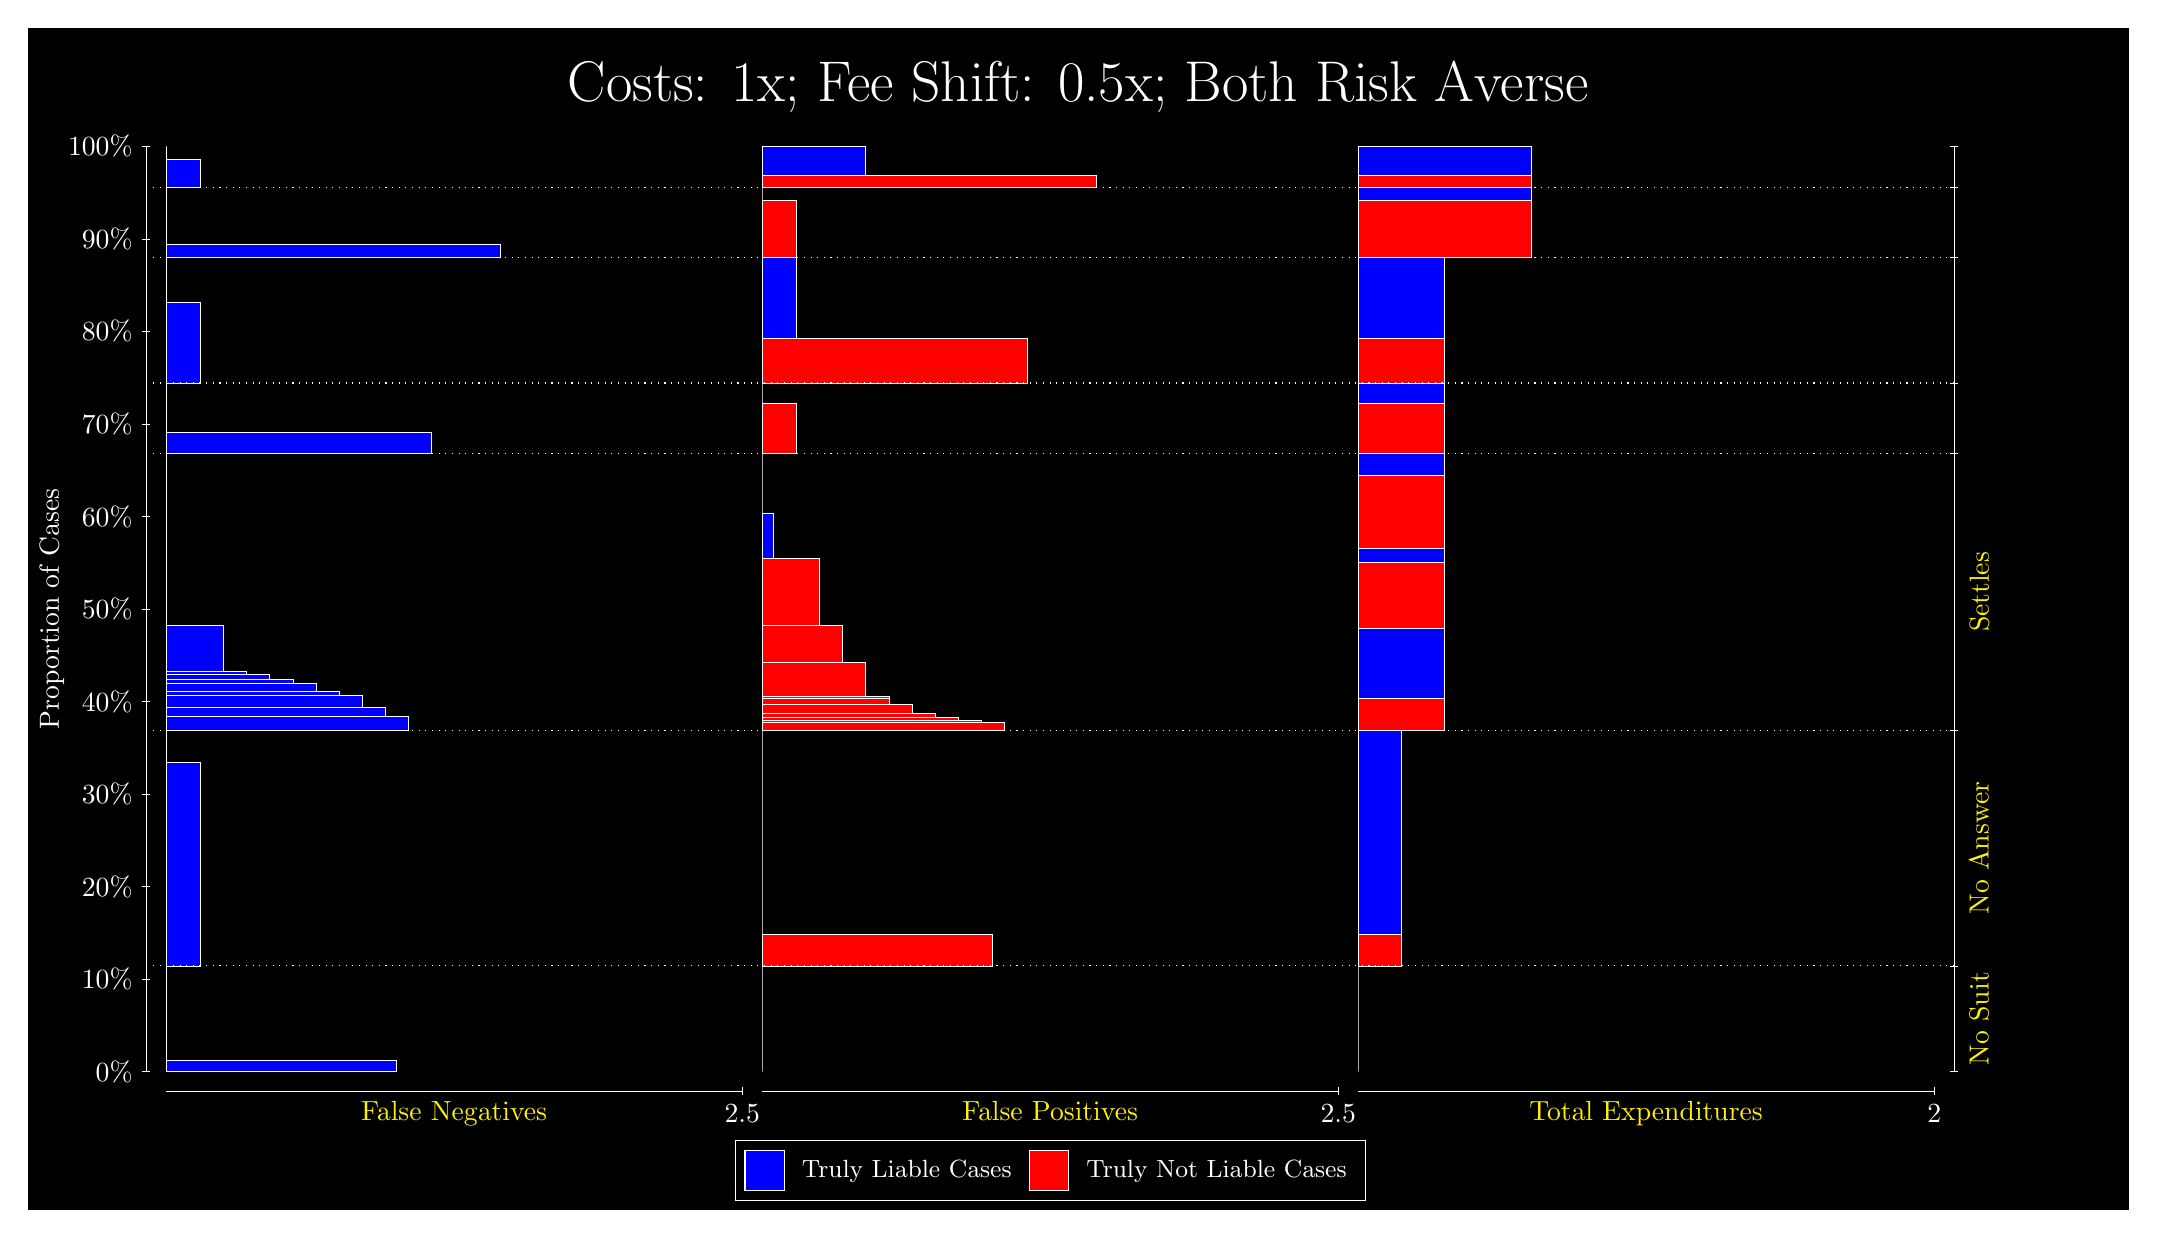
\begin{tikzpicture}
\draw[fill=black] (0,0) rectangle (26.667,15);
\draw[text=white] (0,13.5) rectangle (26.667,15) node[midway] {\huge Costs: 1x; Fee Shift: 0.5x; Both Risk Averse};
\draw[white, very thin] (1.5,1.75) -- (1.5,13.5);
\node[rotate=90, text=white, anchor=center] at (0.3, 7.625) {Proportion of Cases};
\draw[white, very thin] (1.45,1.75) -- (1.55,1.75);
\node[text=white, anchor=east] at (1.45, 1.75) {0\%};
\draw[white, very thin] (1.45,2.925) -- (1.55,2.925);
\node[text=white, anchor=east] at (1.45, 2.925) {10\%};
\draw[white, very thin] (1.45,4.1) -- (1.55,4.1);
\node[text=white, anchor=east] at (1.45, 4.1) {20\%};
\draw[white, very thin] (1.45,5.275) -- (1.55,5.275);
\node[text=white, anchor=east] at (1.45, 5.275) {30\%};
\draw[white, very thin] (1.45,6.45) -- (1.55,6.45);
\node[text=white, anchor=east] at (1.45, 6.45) {40\%};
\draw[white, very thin] (1.45,7.625) -- (1.55,7.625);
\node[text=white, anchor=east] at (1.45, 7.625) {50\%};
\draw[white, very thin] (1.45,8.8) -- (1.55,8.8);
\node[text=white, anchor=east] at (1.45, 8.8) {60\%};
\draw[white, very thin] (1.45,9.975) -- (1.55,9.975);
\node[text=white, anchor=east] at (1.45, 9.975) {70\%};
\draw[white, very thin] (1.45,11.15) -- (1.55,11.15);
\node[text=white, anchor=east] at (1.45, 11.15) {80\%};
\draw[white, very thin] (1.45,12.325) -- (1.55,12.325);
\node[text=white, anchor=east] at (1.45, 12.325) {90\%};
\draw[white, very thin] (1.45,13.5) -- (1.55,13.5);
\node[text=white, anchor=east] at (1.45, 13.5) {100\%};

\draw[white, very thin] (24.457,1.75) -- (24.457,13.5);
\draw[white, very thin] (24.407,1.75) -- (24.507,1.75);
\node[anchor=west] at (24.407, 1.75) {};
\draw[white, very thin] (24.407,3.0925) -- (24.507,3.0925);
\node[anchor=west] at (24.407, 3.0925) {};
\draw[white, very thin] (24.407,6.0832) -- (24.507,6.0832);
\node[anchor=west] at (24.407, 6.0832) {};
\draw[white, very thin] (24.407,9.5995) -- (24.507,9.5995);
\node[anchor=west] at (24.407, 9.5995) {};
\draw[white, very thin] (24.407,10.494) -- (24.507,10.494);
\node[anchor=west] at (24.407, 10.494) {};
\draw[white, very thin] (24.407,12.09) -- (24.507,12.09);
\node[anchor=west] at (24.407, 12.09) {};
\draw[white, very thin] (24.407,12.975) -- (24.507,12.975);
\node[anchor=west] at (24.407, 12.975) {};
\draw[white, very thin] (24.407,13.5) -- (24.507,13.5);
\node[anchor=west] at (24.407, 13.5) {};

\draw[white, very thin, fill=blue] (1.75,1.75) rectangle (4.6775,1.8912);
\draw[white, very thin, fill=red] (1.75,1.8912) rectangle (1.75,3.0925);
\draw[white, very thin, fill=blue] (1.75,3.0925) rectangle (2.1891,5.6782);
\draw[white, very thin, fill=red] (1.75,5.6782) rectangle (1.75,6.0832);
\draw[white, very thin, fill=blue] (1.75,6.0832) rectangle (4.8239,6.2632);
\draw[white, very thin, fill=blue] (1.75,6.2632) rectangle (4.5312,6.3818);
\draw[white, very thin, fill=blue] (1.75,6.3818) rectangle (4.2384,6.5233);
\draw[white, very thin, fill=blue] (1.75,6.5233) rectangle (3.9457,6.577);
\draw[white, very thin, fill=blue] (1.75,6.577) rectangle (3.6529,6.6772);
\draw[white, very thin, fill=blue] (1.75,6.6772) rectangle (3.3602,6.7333);
\draw[white, very thin, fill=blue] (1.75,6.7333) rectangle (3.0674,6.7912);
\draw[white, very thin, fill=blue] (1.75,6.7912) rectangle (2.7746,6.8393);
\draw[white, very thin, fill=blue] (1.75,6.8393) rectangle (2.4819,7.4196);
\draw[white, very thin, fill=red] (1.75,7.4196) rectangle (1.75,9.5995);
\draw[white, very thin, fill=blue] (1.75,9.5995) rectangle (5.1167,9.8626);
\draw[white, very thin, fill=red] (1.75,9.8626) rectangle (1.75,10.494);
\draw[white, very thin, fill=blue] (1.75,10.494) rectangle (2.1891,11.516);
\draw[white, very thin, fill=red] (1.75,11.516) rectangle (1.75,12.09);
\draw[white, very thin, fill=blue] (1.75,12.09) rectangle (5.9949,12.253);
\draw[white, very thin, fill=red] (1.75,12.253) rectangle (1.75,12.975);
\draw[white, very thin, fill=blue] (1.75,12.975) rectangle (2.1891,13.339);
\draw[white, very thin, fill=red] (1.75,13.339) rectangle (1.75,13.5);
\draw[white, very thin, fill=red] (9.3189,1.75) rectangle (9.3189,2.9512);
\draw[white, very thin, fill=blue] (9.3189,2.9512) rectangle (9.3189,3.0925);
\draw[white, very thin, fill=red] (9.3189,3.0925) rectangle (12.246,3.4975);
\draw[white, very thin, fill=blue] (9.3189,3.4975) rectangle (9.3189,6.0832);
\draw[white, very thin, fill=red] (9.3189,6.0832) rectangle (12.393,6.1876);
\draw[white, very thin, fill=red] (9.3189,6.1876) rectangle (12.1,6.2144);
\draw[white, very thin, fill=red] (9.3189,6.2144) rectangle (11.807,6.2497);
\draw[white, very thin, fill=red] (9.3189,6.2497) rectangle (11.515,6.3004);
\draw[white, very thin, fill=red] (9.3189,6.3004) rectangle (11.222,6.4157);
\draw[white, very thin, fill=red] (9.3189,6.4157) rectangle (10.929,6.4895);
\draw[white, very thin, fill=red] (9.3189,6.4895) rectangle (10.929,6.5129);
\draw[white, very thin, fill=red] (9.3189,6.5129) rectangle (10.636,6.9438);
\draw[white, very thin, fill=red] (9.3189,6.9438) rectangle (10.344,7.4155);
\draw[white, very thin, fill=red] (9.3189,7.4155) rectangle (10.051,8.2631);
\draw[white, very thin, fill=blue] (9.3189,8.2631) rectangle (9.4652,8.8434);
\draw[white, very thin, fill=blue] (9.3189,8.8434) rectangle (9.3189,9.5995);
\draw[white, very thin, fill=red] (9.3189,9.5995) rectangle (9.758,10.231);
\draw[white, very thin, fill=blue] (9.3189,10.231) rectangle (9.3189,10.494);
\draw[white, very thin, fill=red] (9.3189,10.494) rectangle (12.686,11.068);
\draw[white, very thin, fill=blue] (9.3189,11.068) rectangle (9.758,12.09);
\draw[white, very thin, fill=red] (9.3189,12.09) rectangle (9.758,12.812);
\draw[white, very thin, fill=blue] (9.3189,12.812) rectangle (9.3189,12.975);
\draw[white, very thin, fill=red] (9.3189,12.975) rectangle (13.564,13.136);
\draw[white, very thin, fill=blue] (9.3189,13.136) rectangle (10.636,13.5);
\draw[white, very thin, fill=red] (16.888,1.75) rectangle (16.888,2.9512);
\draw[white, very thin, fill=blue] (16.888,2.9512) rectangle (16.888,3.0925);
\draw[white, very thin, fill=red] (16.888,3.0925) rectangle (17.437,3.4975);
\draw[white, very thin, fill=blue] (16.888,3.4975) rectangle (17.437,6.0832);
\draw[white, very thin, fill=red] (16.888,6.0832) rectangle (17.986,6.4895);
\draw[white, very thin, fill=blue] (16.888,6.4895) rectangle (17.986,7.3739);
\draw[white, very thin, fill=red] (16.888,7.3739) rectangle (17.986,8.2216);
\draw[white, very thin, fill=blue] (16.888,8.2216) rectangle (17.986,8.4015);
\draw[white, very thin, fill=red] (16.888,8.4015) rectangle (17.986,9.3276);
\draw[white, very thin, fill=blue] (16.888,9.3276) rectangle (17.986,9.5995);
\draw[white, very thin, fill=red] (16.888,9.5995) rectangle (17.986,10.231);
\draw[white, very thin, fill=blue] (16.888,10.231) rectangle (17.986,10.494);
\draw[white, very thin, fill=red] (16.888,10.494) rectangle (17.986,11.068);
\draw[white, very thin, fill=blue] (16.888,11.068) rectangle (17.986,12.09);
\draw[white, very thin, fill=red] (16.888,12.09) rectangle (19.083,12.812);
\draw[white, very thin, fill=blue] (16.888,12.812) rectangle (19.083,12.975);
\draw[white, very thin, fill=red] (16.888,12.975) rectangle (19.083,13.136);
\draw[white, very thin, fill=blue] (16.888,13.136) rectangle (19.083,13.5);
\draw[white, dotted] (1.5,3.0925) -- (24.457,3.0925);
\draw[white, dotted] (1.5,6.0832) -- (24.457,6.0832);
\draw[white, dotted] (1.5,9.5995) -- (24.457,9.5995);
\draw[white, dotted] (1.5,10.494) -- (24.457,10.494);
\draw[white, dotted] (1.5,12.09) -- (24.457,12.09);
\draw[white, dotted] (1.5,12.975) -- (24.457,12.975);
\draw[white, very thin] (1.75,1.5) -- (9.0689,1.5);
\node[text=yellow, anchor=north] at (5.4094, 1.5) {False Negatives};
\draw[white, very thin] (9.0689,1.45) -- (9.0689,1.55);
\node[text=white, anchor=north] at (9.0689, 1.45) {2.5};

\draw[white, very thin] (9.3189,1.5) -- (16.638,1.5);
\node[text=yellow, anchor=north] at (12.978, 1.5) {False Positives};
\draw[white, very thin] (16.638,1.45) -- (16.638,1.55);
\node[text=white, anchor=north] at (16.638, 1.45) {2.5};

\draw[white, very thin] (16.888,1.5) -- (24.207,1.5);
\node[text=yellow, anchor=north] at (20.547, 1.5) {Total Expenditures};
\draw[white, very thin] (24.207,1.45) -- (24.207,1.55);
\node[text=white, anchor=north] at (24.207, 1.45) {2};

\node[text=yellow, centered, rotate=90] at (24.777, 2.4212) {No Suit};
\node[text=yellow, centered, rotate=90] at (24.777, 4.5878) {No Answer};
\node[text=yellow, centered, rotate=90] at (24.777, 7.8414) {Settles};





\draw (12.978300999999998,1.5) node[draw=none] (baseCoordinate) {};
\begin{scope}[align=center]
        \matrix[scale=0.5, draw=white, below=0.5cm of baseCoordinate, nodes={draw}, column sep=0.1cm]{
            \node[rectangle, draw, minimum width=0.5cm, minimum height=0.5cm, fill=blue] {}; &
            \node[draw=none, font=\small, text=white] (B) {Truly Liable Cases}; &
            \node[rectangle, draw, minimum width=0.5cm, minimum height=0.5cm, fill=red] {}; &
            \node[draw=none, font=\small, text=white] (B) {Truly Not Liable Cases}; \\
            };
\end{scope}

\end{tikzpicture}
\end{document}